\documentclass[10pt]{article}
\usepackage[a4paper, top=1.4cm, bottom=1.4cm, left=1.5cm, right=1.5cm]{geometry}
\usepackage{fontspec}
\usepackage{xcolor}
\usepackage{graphicx}
\usepackage{multicol}

\definecolor{vinylpaper}{HTML}{F6EFE2}
\definecolor{vinylink}{HTML}{1C140E}
\definecolor{vinylrust}{HTML}{8C3B2B}
\definecolor{vinylochre}{HTML}{B57B3A}
\definecolor{vinylmuted}{HTML}{5E4D3B}
\definecolor{vinyldark}{HTML}{140F0B}

\setmainfont{Baskerville}[Ligatures=TeX, Scale=0.98]
\setsansfont{Helvetica Neue}[Scale=0.92]
\setmonofont{Courier New Bold}[Scale=0.86]

\setlength{\parindent}{0pt}
\setlength{\parskip}{3pt}
\setlength{\columnsep}{0.9cm}
\pagestyle{empty}

\newcommand{\pageheader}[1]{%
  \noindent{\texttt{\scriptsize\color{vinylmuted} GRAVETOS NO ESCURO — SONGBOOK DE CIFRAS \& HARMONIA}\hfill\texttt{\scriptsize\color{vinylmuted} #1}}\par
  \vspace{-0.15cm}
  \noindent{\color{vinylochre}\rule{\textwidth}{0.5pt}}\par
  \vspace{0.15cm}
}

\begin{document}

% ============================================================================
% CAPA DO SONGBOOK
% ============================================================================
\pagecolor{vinyldark}
\color{vinylpaper}
\begin{center}
  \vspace*{0.6cm}
  {\texttt{\small\color{vinylochre} CADERNO DE CIFRAS, HARMONIA, LEVADAS \& BASTIDORES MUSICAIS}}\par
  \vspace{0.3cm}
  {\Huge\bfseries\color{vinylpaper} SONGBOOK}\par
  \vspace{0.15cm}
  {\LARGE\color{vinylochre} GRAVETOS NO ESCURO}\par
  \vspace{0.5cm}
  \setlength{\fboxsep}{2pt}
  \setlength{\fboxrule}{1.2pt}
  \fcolorbox{vinylochre}{vinyldark}{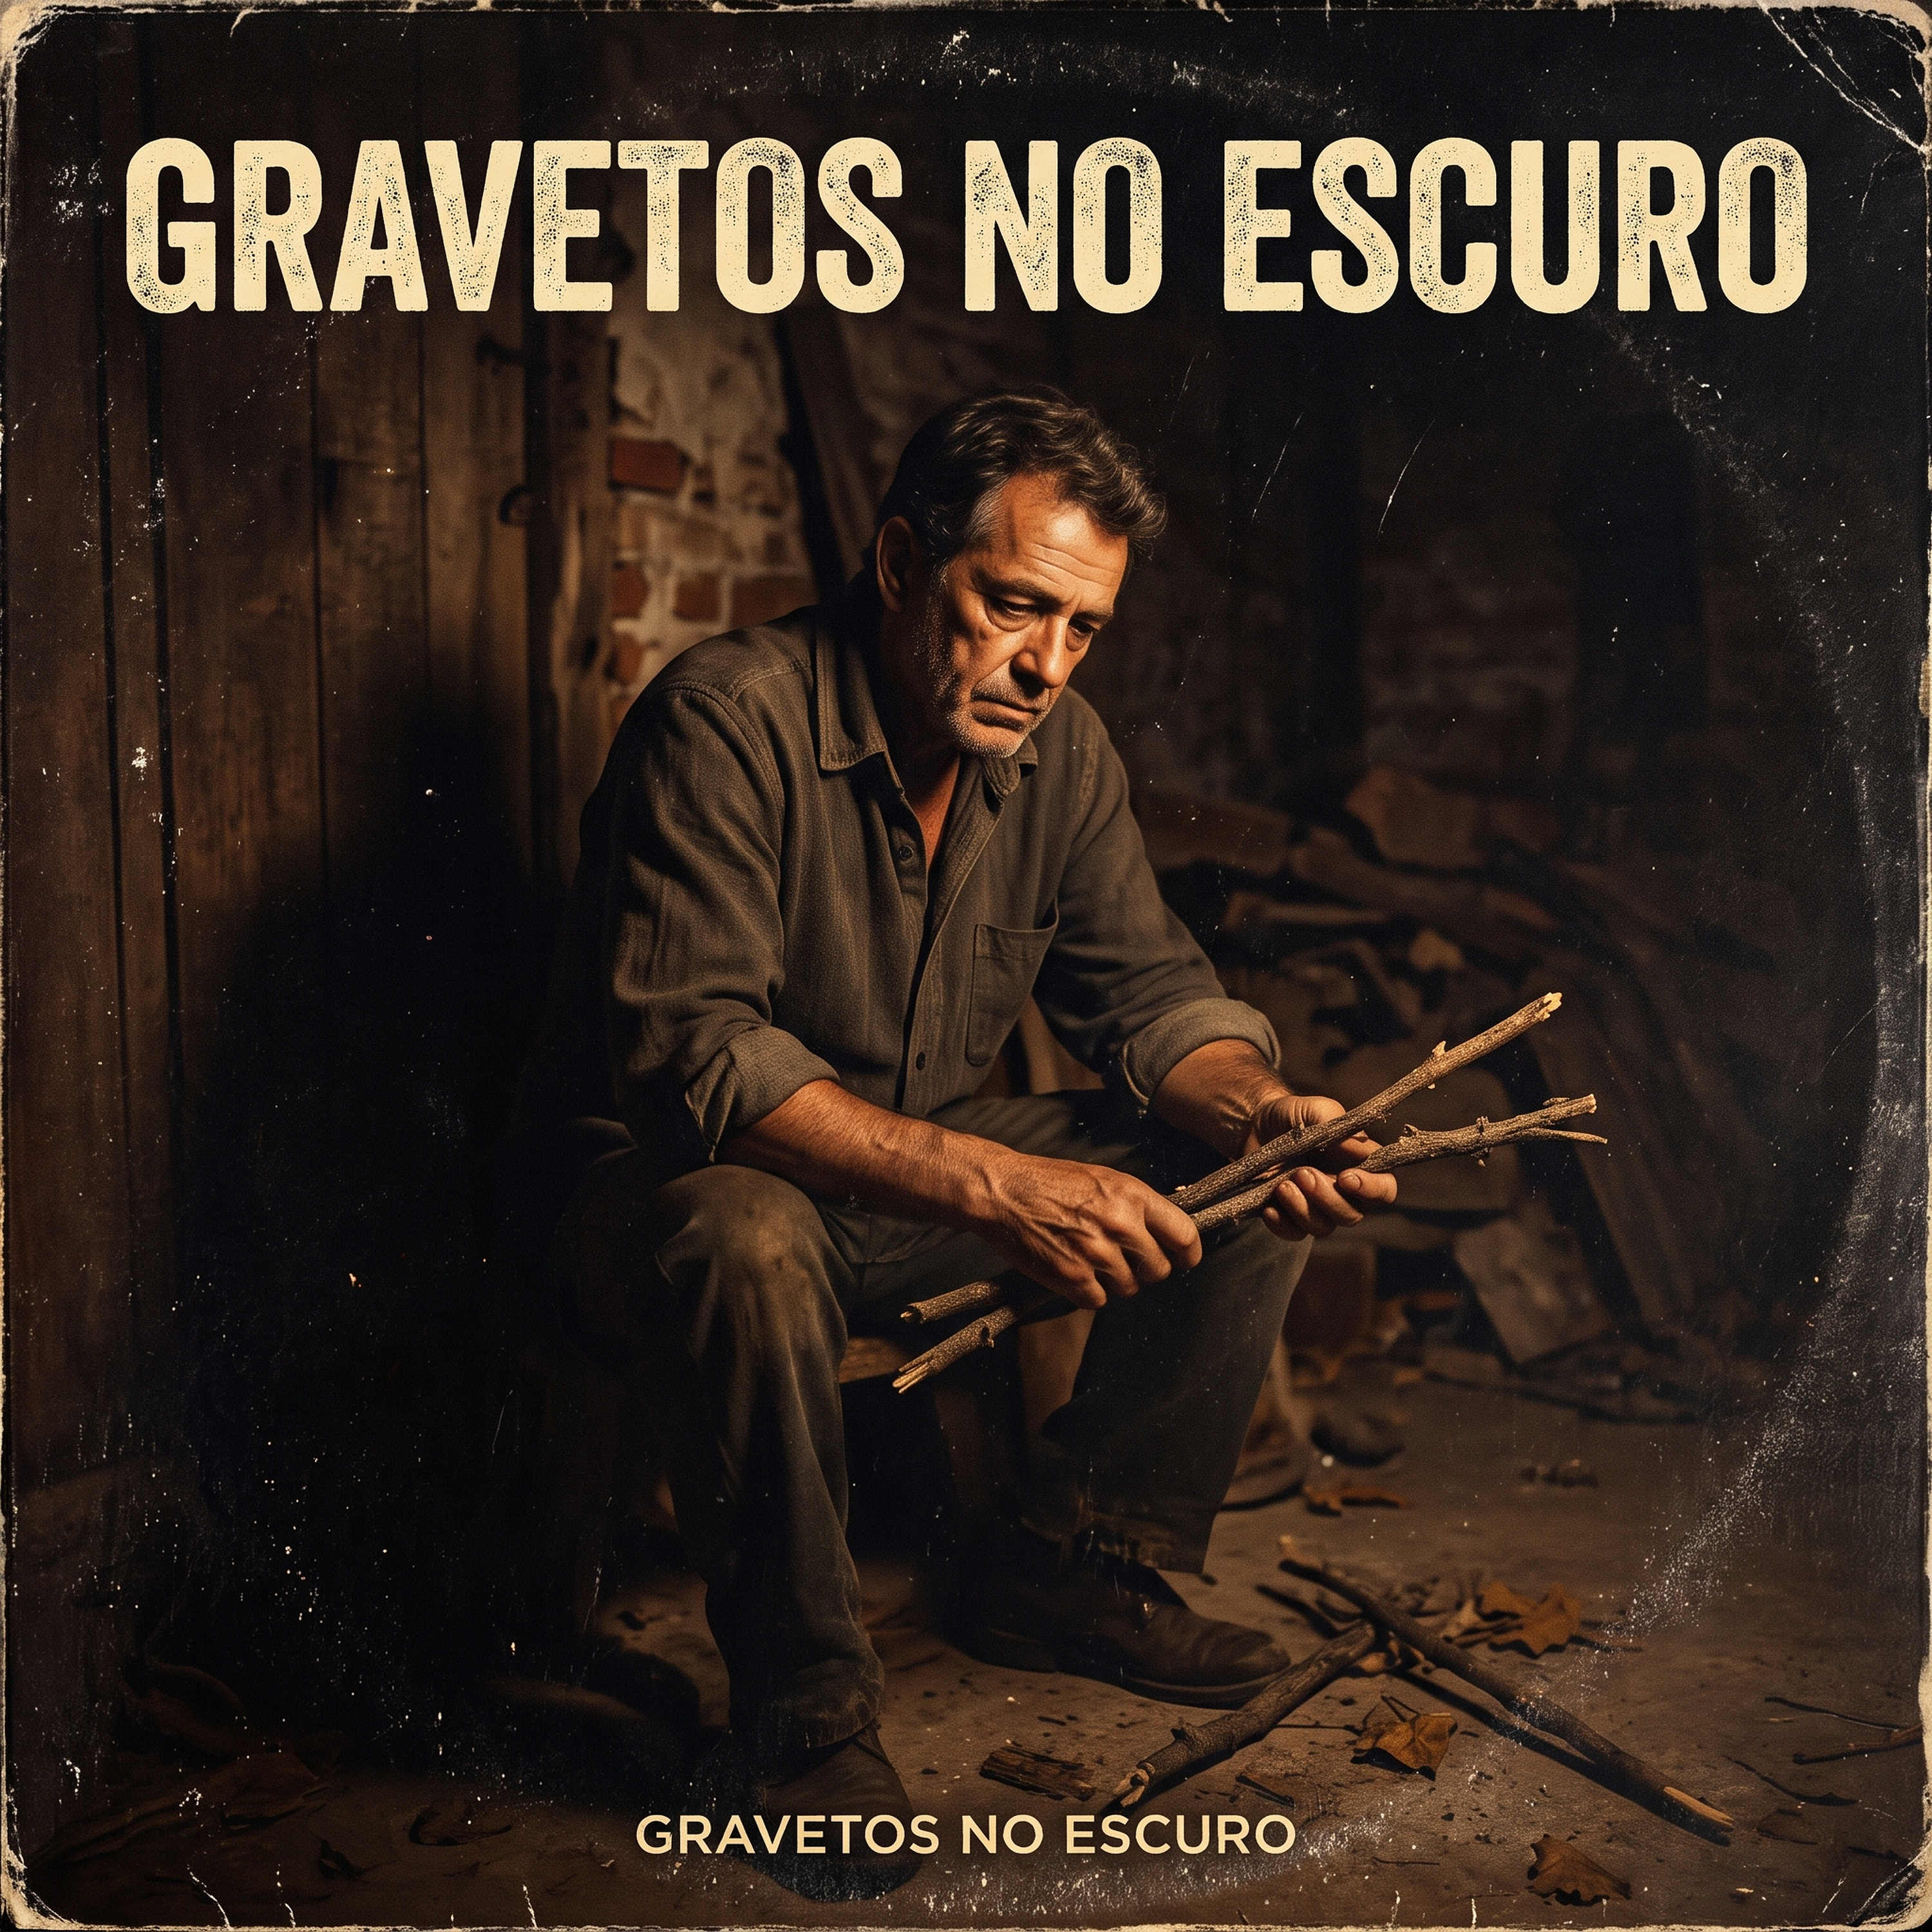
\includegraphics[width=14.8cm, height=14.8cm]{cover-3000x3000.jpg}}\par
  \vspace{0.55cm}
  {\texttt{\footnotesize\color{vinylpaper} 9 FAIXAS CIFRADAS (MPB / SAMBA-CANÇÃO / SAMBA-ROCK-GROOVE)}}\par
  \vspace{0.15cm}
  {\itshape\small\color{vinylochre} “Para quem quiser olhar por trás da cortina: os tons, os acordes e o compasso da travessia.”}\par
  \vspace{0.4cm}
  {\texttt{\scriptsize\color{vinylmuted} EDIÇÃO JUKEBOX $\cdot$ LICENÇA CC BY-SA 4.0}}
\end{center}
\newpage

% ============================================================================
% PÁGINA 2: ÍNDICE HARMÔNICO E MAPA DE TONALIDADES DO LP
% ============================================================================
\pagecolor{vinylpaper}
\color{vinylink}
\pageheader{MAPA HARMÔNICO DO ÁLBUM}

\begin{center}
  {\LARGE\bfseries\color{vinylrust} POR TRÁS DA CORTINA — ARQUITETURA MUSICAL DO LP}\par
  \vspace{0.1cm}
  {\color{vinylrust}\rule{\textwidth}{1.2pt}}
\end{center}

\vspace{0.2cm}
O arco dramático de \textbf{Gravetos no Escuro} foi desenhado não apenas nas letras, mas também no caminho das tonalidades e dos andamentos ao longo dos dois lados do vinil:

\begin{itemize}
  \item \textbf{O Ciclo Menor do Lado A (G\#m $\rightarrow$ C\#m $\rightarrow$ D\#m):} O disco abre em \texttt{G\#m} (68 BPM) no violão de nylon em \textit{Herança de Sal}, acelera para o modo Dórico em 115 BPM em \textit{A Máscara Racha}, passa pela ironia de dominantes secundários em \texttt{C\#m} em \textit{O Intruso de Terno}, e mergulha no registro grave de \texttt{D\#m} (80 BPM) em \textit{Partiu Sem Sair do Lugar}, encerrando o Lado A com 3.5 segundos de silêncio dramático.
  \item \textbf{A Abertura Solar do Lado B (C\#m / E7M $\rightarrow$ Bbm / Db7M $\rightarrow$ G\#m / E7M):} Ao virar o disco, \textit{Âncora no Olhar} inicia em \texttt{C\#m7} mas abre seu refrão no relativo maior luminoso \texttt{E7M}, preparando o terreno para o Samba-Rock Soul solar de \textit{A Ponte Que Não Quebra}. Na faixa 08 (\textit{O Nosso Altar}), a batuqueira sobe para \texttt{Bbm7 / Db7M}, e o álbum fecha o círculo em \textit{Isso é um Túnel} (65 BPM), reconciliando \texttt{G\#m7} e \texttt{E7M}.
\end{itemize}

\vspace{0.3cm}
\noindent{\large\bfseries\color{vinylrust} QUADRO GERAL DAS 9 FAIXAS (TOM ORIGINAL vs. VIOLÃO COM CAPO)}\par
\vspace{0.15cm}
\noindent{\color{vinylochre}\rule{\textwidth}{0.8pt}}\par
\vspace{0.15cm}

\noindent\texttt{\footnotesize\bfseries\color{vinylrust} FAIXA \hfill TOM ORIGINAL \hfill COMPASSO / BPM \hfill SUGESTÃO VIOLÃO / CAPO}\par
\vspace{0.08cm}
\noindent{\color{vinylochre}\rule{\textwidth}{0.4pt}}\par

\noindent\textbf{01. Herança de Sal} \dotfill \texttt{G\#m} \dotfill \texttt{2/4 (68 BPM)} \dotfill \textit{Capo 4ª casa (Em) ou +1 st (Am)}\par\vspace{0.12cm}
\noindent\textbf{02. A Máscara Racha} \dotfill \texttt{G\#m Dórico} \dotfill \texttt{4/4 (115 BPM)} \dotfill \textit{Transpor +1 st (Am7 / D7(9))}\par\vspace{0.12cm}
\noindent\textbf{03. O Intruso de Terno} \dotfill \texttt{C\#m} \dotfill \texttt{2/4 (100 BPM)} \dotfill \textit{Capo 4ª casa (Am)}\par\vspace{0.12cm}
\noindent\textbf{04. O Saldo Não Dá} \dotfill \texttt{G\#m / B7M} \dotfill \texttt{4/4 (90 BPM)} \dotfill \textit{Capo 4ª casa (Em / G7M)}\par\vspace{0.12cm}
\noindent\textbf{05. Partiu Sem Sair do Lugar} \dotfill \texttt{D\#m} \dotfill \texttt{4/4 (80 BPM)} \dotfill \textit{Transpor -1 st (Dm) ou +1 st (Em)}\par\vspace{0.12cm}
\noindent\textbf{06. Âncora no Olhar} \dotfill \texttt{C\#m / E7M} \dotfill \texttt{2/4 (75 BPM)} \dotfill \textit{Capo 4ª casa (Am / C7M)}\par\vspace{0.12cm}
\noindent\textbf{07. A Ponte Que Não Quebra} \dotfill \texttt{E7M / C\#m7} \dotfill \texttt{4/4 (100 BPM)} \dotfill \textit{Posição original (E7M aberto)}\par\vspace{0.12cm}
\noindent\textbf{08. O Nosso Altar} \dotfill \texttt{Bbm7 / Db7M} \dotfill \texttt{4/4 (102 BPM)} \dotfill \textit{Capo 1ª casa (Am7 / C7M)}\par\vspace{0.12cm}
\noindent\textbf{09. Isso é um Túnel} \dotfill \texttt{G\#m7 / E7M} \dotfill \texttt{4/4 (65 BPM)} \dotfill \textit{Capo 4ª casa (Em7 / C7M)}\par

\vfill
\begin{center}
  {\color{vinylochre}\rule{\textwidth}{0.6pt}}\par\vspace{0.1cm}
  {\itshape\footnotesize\color{vinylmuted} Na Jukebox Web (https://raffaine.github.io/jukebox/), use os botões de Transposição (-1 / +1 semitom) para ajustar qualquer cifra em tempo real.}
\end{center}
\newpage


% ============================================================================
% FAIXA 01: HERANÇA DE SAL
% ============================================================================
\pageheader{SONGBOOK OFICIAL $\cdot$ FAIXA 01 (LADO A)}

\noindent{\color{vinylrust}\rule{\textwidth}{1.5pt}}\par\vspace{0.1cm}
\noindent{\LARGE\bfseries\color{vinylink} 01. Herança de Sal}\hfill{\texttt{\small\color{vinylrust} TOM: G\#m $\cdot$ 68 BPM $\cdot$ 2/4 (Samba-Canção Lento)}}\par
\vspace{0.06cm}
\noindent{\texttt{\footnotesize\color{vinylmuted} ESTILO: MPB / Samba-Canção \quad|\quad DICA VIOLÃO: Capo na 4ª casa (tocar em Em) ou afinação 1/2 tom abaixo (Am)}}\par
\vspace{0.1cm}
\noindent{\color{vinylochre}\rule{\textwidth}{0.5pt}}\par
\vspace{0.15cm}

\noindent{\texttt{\scriptsize\color{vinylrust} POR TRÁS DA CORTINA (HARMONIA \& ARRANJO):}}\par
\noindent{\itshape\footnotesize\color{vinylink} A faixa abre o disco em Sol Sustenido Menor (G\#m), uma tonalidade historicamente associada ao lamento contido no violão brasileiro. O ciclo de quartas (G\#m7 $\rightarrow$ C\#m7 $\rightarrow$ F\#7 $\rightarrow$ B7M) cria uma sensação de tentativa de saída para o relativo maior (Si Maior), mas a harmonia sempre é puxada de volta ao chão pelo II–V menor (A\#m7(b5) $\rightarrow$ D\#7(b9)), espelhando a letra onde "nenhum afeto consegue secar" o rio de sombra.}\par
\vspace{0.12cm}
\noindent{\texttt{\scriptsize\color{vinylmuted} LEVADA / GROOVE:}} {\footnotesize\color{vinylink} Rubato intimista no violão de 7 cordas / nylon, com baixarias descendentes em semicolcheias.}\par
\vspace{0.08cm}
\noindent{\texttt{\scriptsize\color{vinylmuted} VOICINGS PRINCIPAIS:}} \texttt{\textbf{G\#m7}} \quad \texttt{\textbf{C\#m7}} \quad \texttt{\textbf{F\#7(13)}} \quad \texttt{\textbf{B7M}} \quad \texttt{\textbf{E7M}} \quad \texttt{\textbf{A\#m7(b5)}} \quad \texttt{\textbf{D\#7(b9)}}\par
\vspace{0.15cm}
\noindent{\color{vinylochre}\rule{\textwidth}{0.5pt}}

\begin{multicols}{2}
\setlength{\parskip}{1pt}
\vspace{0.12cm}\noindent{\texttt{\footnotesize\bfseries\color{vinylrust} [Intro] G\#m7  C\#m7  A\#m7(b5)  D\#7(b9)  G\#m7}}

\vspace{0.16cm}

\vspace{0.12cm}\noindent{\texttt{\footnotesize\bfseries\color{vinylrust} [Primeira Parte]}}

\noindent{\texttt{\footnotesize\bfseries\color{vinylrust}G\#m7~~~~~~~~~~~~~~~~~~~~~~~~C\#m7}}

\noindent{\rmfamily\small\color{vinylink}Nasci sozinho na beira da estrada}

\noindent{\texttt{\footnotesize\bfseries\color{vinylrust}D\#7(b9)~~~~~~~~~~~~~~~~~~~~~G\#m7}}

\noindent{\rmfamily\small\color{vinylink}Sem muita história nem fado pra rir}

\noindent{\texttt{\footnotesize\bfseries\color{vinylrust}G\#m7~~~~~~~~~~~~~~~~~~~~~~~~C\#m7}}

\noindent{\rmfamily\small\color{vinylink}A infância escassa me deu quase nada}

\noindent{\texttt{\footnotesize\bfseries\color{vinylrust}F\#7(13)~~~~~~~~~~~~~~~~~~~~~B7M}}

\noindent{\rmfamily\small\color{vinylink}E a dor foi a mestra pra me conduzir}

\noindent{\texttt{\footnotesize\bfseries\color{vinylrust}E7M~~~~~~~~~~~~~~~~~~~~~~~~~A\#m7(b5)}}

\noindent{\rmfamily\small\color{vinylink}Fiquei sem meu mundo perdi meu norte}

\noindent{\texttt{\footnotesize\bfseries\color{vinylrust}D\#7(b9)~~~~~~~~~~~~~~~~~~~~~G\#m7}}

\noindent{\rmfamily\small\color{vinylink}Canto baixinho o que a vida calou}

\noindent{\texttt{\footnotesize\bfseries\color{vinylrust}E7M~~~~~~~~~~~~~~~~~~~~~~~~~A\#m7(b5)}}

\noindent{\rmfamily\small\color{vinylink}Catando gravetos driblando a sorte}

\noindent{\texttt{\footnotesize\bfseries\color{vinylrust}D\#7(b9)~~~~~~~~~~~~~~~~~~~~~G\#m7}}

\noindent{\rmfamily\small\color{vinylink}Sou a exceção que o tempo esqueceu}

\vspace{0.16cm}

\vspace{0.12cm}\noindent{\texttt{\footnotesize\bfseries\color{vinylrust} [Refrão]}}

\noindent{\texttt{\footnotesize\bfseries\color{vinylrust}~~~~~~~~~~~~C\#m7~~~~~~~~~~~~~~~~F\#7(13)}}

\noindent{\rmfamily\small\color{vinylink}A solidão é herança sem fim}

\noindent{\texttt{\footnotesize\bfseries\color{vinylrust}~~~~~~~~~~~~B7M~~~~~~~~~~~~~~~~~E7M}}

\noindent{\rmfamily\small\color{vinylink}Mora no fundo e não sai de mim}

\noindent{\texttt{\footnotesize\bfseries\color{vinylrust}~~~~~~~~~~~~A\#m7(b5)~~~~~~~~~~~~D\#7(b9)}}

\noindent{\rmfamily\small\color{vinylink}Um rio de sombra que quer me afogar}

\noindent{\texttt{\footnotesize\bfseries\color{vinylrust}~~~~~~~~~~~~G\#m7~~~~~~~~~~~~~~~~G\#7(b13)}}

\noindent{\rmfamily\small\color{vinylink}E nenhum afeto consegue secar}

\noindent{\texttt{\footnotesize\bfseries\color{vinylrust}~~~~~~~~~~~~C\#m7~~~~~~~~~~~~~~~~D\#7(b9)}}

\noindent{\rmfamily\small\color{vinylink}A canção do vazio que vem me cobrar}

\noindent{\texttt{\footnotesize\bfseries\color{vinylrust}~~~~~~~~~~~~A\#m7(b5)~~D\#7(b9)~~~G\#m7}}

\noindent{\rmfamily\small\color{vinylink}O preço de nunca poder descansar}

\vspace{0.16cm}

\vspace{0.12cm}\noindent{\texttt{\footnotesize\bfseries\color{vinylrust} [Segunda Parte]}}

\noindent{\texttt{\footnotesize\bfseries\color{vinylrust}G\#m7~~~~~~~~~~~~~~~~~~~~~~~~C\#m7}}

\noindent{\rmfamily\small\color{vinylink}O mundo sorriu e me deu um lugar}

\noindent{\texttt{\footnotesize\bfseries\color{vinylrust}F\#7(13)~~~~~~~~~~~~~~~~~~~~~B7M}}

\noindent{\rmfamily\small\color{vinylink}Um novo carinho uma outra mãe}

\noindent{\texttt{\footnotesize\bfseries\color{vinylrust}E7M~~~~~~~~~~~~~~~~~~~~~~~~~A\#m7(b5)}}

\noindent{\rmfamily\small\color{vinylink}Mas logo o destino voltou a roubar}

\noindent{\texttt{\footnotesize\bfseries\color{vinylrust}D\#7(b9)~~~~~~~~~~~~~~~~~~~~~G\#m7}}

\noindent{\rmfamily\small\color{vinylink}A ponte que eu fiz para não naufragar}

\noindent{\texttt{\footnotesize\bfseries\color{vinylrust}G\#m7~~~~~~~~~~~~~~~~~~~~~~~~C\#m7}}

\noindent{\rmfamily\small\color{vinylink}E agora de novo a mesma canção}

\noindent{\texttt{\footnotesize\bfseries\color{vinylrust}F\#7(13)~~~~~~~~~~~~~~~~~~~~~B7M}}

\noindent{\rmfamily\small\color{vinylink}Deitar com o medo no escuro sem fim}

\noindent{\texttt{\footnotesize\bfseries\color{vinylrust}E7M~~~~~~~~~~~~~~~~~~~~~~~~~A\#m7(b5)}}

\noindent{\rmfamily\small\color{vinylink}O cansaço é o mastro dessa embarcação}

\noindent{\texttt{\footnotesize\bfseries\color{vinylrust}D\#7(b9)~~~~~~~~~~~~~~~~~~~~~G\#m7}}

\noindent{\rmfamily\small\color{vinylink}E a lágrima o único sal para mim}

\vspace{0.16cm}

\vspace{0.12cm}\noindent{\texttt{\footnotesize\bfseries\color{vinylrust} [Terceira Parte / Desfecho]}}

\noindent{\texttt{\footnotesize\bfseries\color{vinylrust}G\#m7~~~~~~~~~~~~~~~~~~~~~~~~C\#m7}}

\noindent{\rmfamily\small\color{vinylink}Uma família sorri no meu lar}

\noindent{\texttt{\footnotesize\bfseries\color{vinylrust}F\#7(13)~~~~~~~~~~~~~~~~~~~~~B7M}}

\noindent{\rmfamily\small\color{vinylink}A mesa está posta o beijo me acolhe}

\noindent{\texttt{\footnotesize\bfseries\color{vinylrust}E7M~~~~~~~~~~~~~~~~~~~~~~~~~A\#m7(b5)}}

\noindent{\rmfamily\small\color{vinylink}Mas ela se esconde no canto a espiar}

\noindent{\texttt{\footnotesize\bfseries\color{vinylrust}D\#7(b9)~~~~~~~~~~~~~~~~~~~~~G\#m7}}

\noindent{\rmfamily\small\color{vinylink}Esperando a hora em que a força me encolhe}

\noindent{\texttt{\footnotesize\bfseries\color{vinylrust}E7M~~~~~~~~~~~~~~~~~~~~~~~~~C\#m7}}

\noindent{\rmfamily\small\color{vinylink}Não é desamor não é falta de fé}

\noindent{\texttt{\footnotesize\bfseries\color{vinylrust}A\#m7(b5)~~~~~~~~~~~~~~~~~~~~D\#7(b9)}}

\noindent{\rmfamily\small\color{vinylink}É só que o vazio tem fome de mim}

\noindent{\texttt{\footnotesize\bfseries\color{vinylrust}C\#m7~~~~~~~~~~~~~~~~~~~~~~~~D\#7(b9)}}

\noindent{\rmfamily\small\color{vinylink}Destrói minhas pontes me deixa sem pé}

\noindent{\texttt{\footnotesize\bfseries\color{vinylrust}A\#m7(b5)~~~~~~~~D\#7(b9)~~~~~G\#m7}}

\noindent{\rmfamily\small\color{vinylink}E escreve em silêncio o meu próprio fim}
\end{multicols}
\newpage


% ============================================================================
% FAIXA 02: A MÁSCARA RACHA
% ============================================================================
\pageheader{SONGBOOK OFICIAL $\cdot$ FAIXA 02 (LADO A)}

\noindent{\color{vinylrust}\rule{\textwidth}{1.5pt}}\par\vspace{0.1cm}
\noindent{\LARGE\bfseries\color{vinylink} 02. A Máscara Racha (Máscara no Asfalto)}\hfill{\texttt{\small\color{vinylrust} TOM: G\#m (Dórico) $\cdot$ 115 BPM $\cdot$ 4/4 (Funk Brasileiro \& Samba-Rock)}}\par
\vspace{0.06cm}
\noindent{\texttt{\footnotesize\color{vinylmuted} ESTILO: Funk Brasileiro \& Samba-Rock \quad|\quad DICA VIOLÃO: Transpor +1 semitom para tocar em Am7 / D7(9) no violão}}\par
\vspace{0.1cm}
\noindent{\color{vinylochre}\rule{\textwidth}{0.5pt}}\par
\vspace{0.15cm}

\noindent{\texttt{\scriptsize\color{vinylrust} POR TRÁS DA CORTINA (HARMONIA \& ARRANJO):}}\par
\noindent{\itshape\footnotesize\color{vinylink} Depois da introspecção da Faixa 01, a harmonia permanece em G\#m, mas muda do modo Eólio para o modo Dórico (G\#m7 $\leftrightarrow$ C\#7(9)). Esse vamp de dois acordes — marca registrada de Jorge Ben e Tim Maia nos anos 70 — injeta adrenalina imediata. No refrão, a queda cromática E7M $\rightarrow$ D\#7(\#9) (o famoso "acorde Hendrix" de dominante com nona aumentada) traduz a tensão da máscara rachando na madrugada.}\par
\vspace{0.12cm}
\noindent{\texttt{\scriptsize\color{vinylmuted} LEVADA / GROOVE:}} {\footnotesize\color{vinylink} Groove sincopado em 115 BPM com guitarra wah-wah no contratempo e ataque de metais no acorde D\#7(\#9).}\par
\vspace{0.08cm}
\noindent{\texttt{\scriptsize\color{vinylmuted} VOICINGS PRINCIPAIS:}} \texttt{\textbf{G\#m7}} \quad \texttt{\textbf{C\#7(9)}} \quad \texttt{\textbf{E7M}} \quad \texttt{\textbf{D\#7(\#9)}} \quad \texttt{\textbf{B7M}}\par
\vspace{0.15cm}
\noindent{\color{vinylochre}\rule{\textwidth}{0.5pt}}

\begin{multicols}{2}
\setlength{\parskip}{1pt}
\vspace{0.12cm}\noindent{\texttt{\footnotesize\bfseries\color{vinylrust} [Intro / Riff Metais] G\#m7  C\#7(9)  G\#m7  D\#7(\#9)}}

\vspace{0.16cm}

\vspace{0.12cm}\noindent{\texttt{\footnotesize\bfseries\color{vinylrust} [Primeira Parte]}}

\noindent{\texttt{\footnotesize\bfseries\color{vinylrust}G\#m7~~~~~~~~~~~~~~~~~~~~~~~~~~~~~~C\#7(9)}}

\noindent{\rmfamily\small\color{vinylink}Cheguei na cena feito estranho no ninho}

\noindent{\texttt{\footnotesize\bfseries\color{vinylrust}G\#m7~~~~~~~~~~~~~~~~~~~~~~~~~~~~~~C\#7(9)}}

\noindent{\rmfamily\small\color{vinylink}Com a rejeição batendo forte no peito}

\noindent{\texttt{\footnotesize\bfseries\color{vinylrust}G\#m7~~~~~~~~~~~~~~~~~~~~~~~~~~~~~~C\#7(9)}}

\noindent{\rmfamily\small\color{vinylink}Vesti a capa de quem anda sozinho}

\noindent{\texttt{\footnotesize\bfseries\color{vinylrust}E7M~~~~~~~~~~~~~~~~~~~~~~~~~~~~~~~D\#7(\#9)}}

\noindent{\rmfamily\small\color{vinylink}Um outsider com defeito no jeito}

\noindent{\texttt{\footnotesize\bfseries\color{vinylrust}G\#m7~~~~~~~~~~~~~~~~~~~~~~~~~~~~~~C\#7(9)}}

\noindent{\rmfamily\small\color{vinylink}Era a armadura pra esconder a ferida}

\noindent{\texttt{\footnotesize\bfseries\color{vinylrust}G\#m7~~~~~~~~~~~~~~~~~~~~~~~~~~~~~~C\#7(9)}}

\noindent{\rmfamily\small\color{vinylink}A bofetada que a vida me deu}

\noindent{\texttt{\footnotesize\bfseries\color{vinylrust}E7M~~~~~~~~~~~~~~~~~~~~~~~~~~~~~~~C\#m7}}

\noindent{\rmfamily\small\color{vinylink}Criei um personagem pra lida}

\noindent{\texttt{\footnotesize\bfseries\color{vinylrust}D\#7(\#9)~~~~~~~~~~~~~~~~~~~~~~~~~~~G\#m7}}

\noindent{\rmfamily\small\color{vinylink}E o verdadeiro 'eu' se escondeu}

\vspace{0.16cm}

\vspace{0.12cm}\noindent{\texttt{\footnotesize\bfseries\color{vinylrust} [Refrão]}}

\noindent{\texttt{\footnotesize\bfseries\color{vinylrust}G\#m7~~~~~~~~~~~~~~~~~~~~~~~~~~~~~~C\#7(9)}}

\noindent{\rmfamily\small\color{vinylink}Mas a máscara racha quando a noite vem cobrando}

\noindent{\texttt{\footnotesize\bfseries\color{vinylrust}E7M~~~~~~~~~~~~~~~~~~~~~~~~~~~~~~~D\#7(\#9)}}

\noindent{\rmfamily\small\color{vinylink}A solidão não dorme, ela fica só espreitando}

\noindent{\texttt{\footnotesize\bfseries\color{vinylrust}G\#m7~~~~~~~~~~~~~~~~~~~~~~~~~~~~~~C\#7(9)}}

\noindent{\rmfamily\small\color{vinylink}Mudei o rumo, encontrei o meu lugar}

\noindent{\texttt{\footnotesize\bfseries\color{vinylrust}E7M~~~~~~~~~~~~~~~D\#7(\#9)~~~~~~~~~G\#m7}}

\noindent{\rmfamily\small\color{vinylink}Nesse bonde que me ensina a caminhar}

\vspace{0.16cm}

\vspace{0.12cm}\noindent{\texttt{\footnotesize\bfseries\color{vinylrust} [Segunda Parte]}}

\noindent{\texttt{\footnotesize\bfseries\color{vinylrust}G\#m7~~~~~~~~~~~~~~~~~~~~~~~~~~~~~~C\#7(9)}}

\noindent{\rmfamily\small\color{vinylink}Fui queimar a juventude no fogo do escape}

\noindent{\texttt{\footnotesize\bfseries\color{vinylrust}G\#m7~~~~~~~~~~~~~~~~~~~~~~~~~~~~~~C\#7(9)}}

\noindent{\rmfamily\small\color{vinylink}Buscando anestesia pra não ver o estrago}

\noindent{\texttt{\footnotesize\bfseries\color{vinylrust}G\#m7~~~~~~~~~~~~~~~~~~~~~~~~~~~~~~C\#7(9)}}

\noindent{\rmfamily\small\color{vinylink}Abraçando o perigo, jogando no blefe}

\noindent{\texttt{\footnotesize\bfseries\color{vinylrust}E7M~~~~~~~~~~~~~~~~~~~~~~~~~~~~~~~D\#7(\#9)}}

\noindent{\rmfamily\small\color{vinylink}Ouvindo discursos que me punham de lado}

\noindent{\texttt{\footnotesize\bfseries\color{vinylrust}C\#m7~~~~~~~~~~~~~~~~~~~~~~~~~~~~~~G\#m7}}

\noindent{\rmfamily\small\color{vinylink}Olhava pra vitrine e o preço era alto demais}

\noindent{\texttt{\footnotesize\bfseries\color{vinylrust}C\#m7~~~~~~~~~~~~~~~~~~~~~~~~~~~~~~G\#m7}}

\noindent{\rmfamily\small\color{vinylink}Amizades rasas, amores de plástico, sem paz}

\noindent{\texttt{\footnotesize\bfseries\color{vinylrust}E7M~~~~~~~~~~~~~~~~~~~~~~~~~~~~~~~C\#m7}}

\noindent{\rmfamily\small\color{vinylink}Errei por imaturo, perdi conexões no caminho}

\noindent{\texttt{\footnotesize\bfseries\color{vinylrust}D\#7(\#9)}}

\noindent{\rmfamily\small\color{vinylink}Mas era só o medo de morrer sozinho}

\vspace{0.16cm}

\vspace{0.12cm}\noindent{\texttt{\footnotesize\bfseries\color{vinylrust} [Coda / Batuque Final]}}

\noindent{\texttt{\footnotesize\bfseries\color{vinylrust}G\#m7~~~~~~~~~~~~~~~~~~~~~~~~~~~~~~C\#7(9)}}

\noindent{\rmfamily\small\color{vinylink}O cansaço é real, mas o cansaço não me para não}

\noindent{\texttt{\footnotesize\bfseries\color{vinylrust}E7M~~~~~~~~~~~~~~~~~~~~~~~~~~~~~~~D\#7(\#9)}}

\noindent{\rmfamily\small\color{vinylink}A solidão tá aqui, mas agora eu tenho o meu bando}

\noindent{\texttt{\footnotesize\bfseries\color{vinylrust}G\#m7~~~~~~~~~~~~~~~~~~~~~~~~~~~~~~C\#7(9)}}

\noindent{\rmfamily\small\color{vinylink}Samba-rock pesado pra espantar a escuridão}

\noindent{\texttt{\footnotesize\bfseries\color{vinylrust}E7M~~~~~~~~~~~~~~~D\#7(\#9)~~~~~~~~~G\#m7}}

\noindent{\rmfamily\small\color{vinylink}E o monstro do vazio tá de longe só olhando}
\end{multicols}
\newpage


% ============================================================================
% FAIXA 03: O INTRUSO DE TERNO
% ============================================================================
\pageheader{SONGBOOK OFICIAL $\cdot$ FAIXA 03 (LADO A)}

\noindent{\color{vinylrust}\rule{\textwidth}{1.5pt}}\par\vspace{0.1cm}
\noindent{\LARGE\bfseries\color{vinylink} 03. O Intruso de Terno}\hfill{\texttt{\small\color{vinylrust} TOM: C\#m $\cdot$ 100 BPM $\cdot$ 2/4 (Samba de Breque)}}\par
\vspace{0.06cm}
\noindent{\texttt{\footnotesize\color{vinylmuted} ESTILO: Samba de Breque \quad|\quad DICA VIOLÃO: Capo na 4ª casa (tocar em Am) ou +1 semitom (Dm)}}\par
\vspace{0.1cm}
\noindent{\color{vinylochre}\rule{\textwidth}{0.5pt}}\par
\vspace{0.15cm}

\noindent{\texttt{\scriptsize\color{vinylrust} POR TRÁS DA CORTINA (HARMONIA \& ARRANJO):}}\par
\noindent{\itshape\footnotesize\color{vinylink} Construída em Dó Sustenido Menor (C\#m), esta faixa usa dominantes secundários em cadeia (C\#7 $\rightarrow$ F\#m7 $\rightarrow$ B7(9) $\rightarrow$ E7M $\rightarrow$ A7M $\rightarrow$ D\#7(9) $\rightarrow$ G\#7(b13)) para dar o ar teatral e irônico do Samba de Breque clássico de Moreira da Silva. Na última frase ("Cadeira tá vaga? Pois é, agora eu ocupo"), a banda inteira faz um breque seco no G\#7(b13) e só resolve no C\#m6/9 depois da fala.}\par
\vspace{0.12cm}
\noindent{\texttt{\scriptsize\color{vinylmuted} LEVADA / GROOVE:}} {\footnotesize\color{vinylink} Samba malandro em 100 BPM com paradas secas (breques) no G\#7(b13) antes das frases faladas.}\par
\vspace{0.08cm}
\noindent{\texttt{\scriptsize\color{vinylmuted} VOICINGS PRINCIPAIS:}} \texttt{\textbf{C\#m7}} \quad \texttt{\textbf{G\#7(b13)}} \quad \texttt{\textbf{F\#m7}} \quad \texttt{\textbf{B7(9)}} \quad \texttt{\textbf{E7M}} \quad \texttt{\textbf{A7M}} \quad \texttt{\textbf{D\#7(b9)}}\par
\vspace{0.15cm}
\noindent{\color{vinylochre}\rule{\textwidth}{0.5pt}}

\begin{multicols}{2}
\setlength{\parskip}{1pt}
\vspace{0.12cm}\noindent{\texttt{\footnotesize\bfseries\color{vinylrust} [Intro] C\#m7  D\#7(b9)  G\#7(b13)  C\#m7  (Breque!)}}

\vspace{0.16cm}

\vspace{0.12cm}\noindent{\texttt{\footnotesize\bfseries\color{vinylrust} [Primeira Parte]}}

\noindent{\texttt{\footnotesize\bfseries\color{vinylrust}C\#m7~~~~~~~~~~~~~~~~~~~~~~~~~~~~~~G\#7(b13)}}

\noindent{\rmfamily\small\color{vinylink}Entrei sem bater a porta tava encostada}

\noindent{\texttt{\footnotesize\bfseries\color{vinylrust}C\#m7~~~~~~~~~~~~~~~~~~~~~~~~~~~~~~F\#m7}}

\noindent{\rmfamily\small\color{vinylink}A mesa cheia de gente a alma bem guardada}

\noindent{\texttt{\footnotesize\bfseries\color{vinylrust}F\#m7~~~~~~~~~~~~~~~~~~~~~~~~~~~~~~B7(9)}}

\noindent{\rmfamily\small\color{vinylink}Comentei do vinho dei risada do azar}

\noindent{\texttt{\footnotesize\bfseries\color{vinylrust}E7M~~~~~~~~~~~~~~~~~~~~~~~~~~~~~~~G\#7(b13)}}

\noindent{\rmfamily\small\color{vinylink}Notei que ninguém nota quem não quer se ajustar}

\noindent{\texttt{\footnotesize\bfseries\color{vinylrust}C\#m7~~~~~~~~~~~~~~~~~~~~~~~~~~~~~~G\#7(b13)}}

\noindent{\rmfamily\small\color{vinylink}O garçom me olha o anfitrião não conhece}

\noindent{\texttt{\footnotesize\bfseries\color{vinylrust}F\#m7~~~~~~~~~~~~~~~~~~~~~~~~~~~~~~B7(9)}}

\noindent{\rmfamily\small\color{vinylink}Mas esse é o meu charme é assim que a vida floresce}

\noindent{\texttt{\footnotesize\bfseries\color{vinylrust}A7M~~~~~~~~~~~~~~~~~~~~~~~~~~~~~~~G\#7(b13)}}

\noindent{\rmfamily\small\color{vinylink}Fingem que não veem mas eu tô no salão}

\noindent{\texttt{\footnotesize\bfseries\color{vinylrust}C\#m7~~~~~~~~~~~~~~G\#7(b13)~~~~~~~~C\#m7}}

\noindent{\rmfamily\small\color{vinylink}O intruso de terno o dono da situação}

\vspace{0.16cm}

\vspace{0.12cm}\noindent{\texttt{\footnotesize\bfseries\color{vinylrust} [Segunda Parte]}}

\noindent{\texttt{\footnotesize\bfseries\color{vinylrust}C\#m7~~~~~~~~~~~~~~~~~~~~~~~~~~~~~~G\#7(b13)}}

\noindent{\rmfamily\small\color{vinylink}Aponto o dedo pro destino ele me olha com raiva}

\noindent{\texttt{\footnotesize\bfseries\color{vinylrust}C\#m7~~~~~~~~~~~~~~~~~~~~~~~~~~~~~~F\#m7}}

\noindent{\rmfamily\small\color{vinylink}Eu sou o erro do sistema a peça que se lava}

\noindent{\texttt{\footnotesize\bfseries\color{vinylrust}B7(9)~~~~~~~~~~~~~~~~~~~~~~~~~~~~~E7M}}

\noindent{\rmfamily\small\color{vinylink}Mas não sai a mancha eu sou o risco no cristal}

\noindent{\texttt{\footnotesize\bfseries\color{vinylrust}A7M~~~~~~~~~~~~~~~~~~~~~~~~~~~~~~~G\#7(b13)}}

\noindent{\rmfamily\small\color{vinylink}Quem nasceu pra exceção não se sente mal no carnaval}

\noindent{\texttt{\footnotesize\bfseries\color{vinylrust}F\#m7~~~~~~~~~~~~~~~~~~~~~~~~~~~~~~C\#m7}}

\noindent{\rmfamily\small\color{vinylink}Sorrio o sorriso que todo mundo prefere}

\noindent{\texttt{\footnotesize\bfseries\color{vinylrust}D\#7(b9)~~~~~~~~~~~~~~~~~~~~~~~~~~~G\#7(b13)}}

\noindent{\rmfamily\small\color{vinylink}Enquanto o meu cínico interior se diverte}

\noindent{\texttt{\footnotesize\bfseries\color{vinylrust}F\#m7~~~~~~~~~~~~~~~~~~~~~~~~~~~~~~C\#m7}}

\noindent{\rmfamily\small\color{vinylink}Vendo a vida de vocês com esse medo de cair}

\noindent{\texttt{\footnotesize\bfseries\color{vinylrust}A7M~~~~~~~~~~~~~~~~~~~~~~~~~~~~~~~G\#7(b13)~~~(Breque!)}}

\noindent{\rmfamily\small\color{vinylink}Eu já tô no chão meu amigo não tenho pra onde fugir}

\vspace{0.16cm}

\vspace{0.12cm}\noindent{\texttt{\footnotesize\bfseries\color{vinylrust} [Refrão]}}

\noindent{\texttt{\footnotesize\bfseries\color{vinylrust}C\#m7~~~~~~~~~~~~~~~~~~~~~~~~~~~~~~F\#m7}}

\noindent{\rmfamily\small\color{vinylink}É o dedo do meio pro que o mundo desenhou!}

\noindent{\texttt{\footnotesize\bfseries\color{vinylrust}B7(9)~~~~~~~~~~~~~~~~~~~~~~~~~~~~~E7M}}

\noindent{\rmfamily\small\color{vinylink}Eu sou o convidado que o dono não chamou!}

\noindent{\texttt{\footnotesize\bfseries\color{vinylrust}A7M~~~~~~~~~~~~~~~~~~~~~~~~~~~~~~~F\#m7}}

\noindent{\rmfamily\small\color{vinylink}Pode fechar a porta eu entro pela janela!}

\noindent{\texttt{\footnotesize\bfseries\color{vinylrust}D\#7(b9)~~~~~~~~~~~~~~~~~~~~~~~~~~~G\#7(b13)}}

\noindent{\rmfamily\small\color{vinylink}A vida é esse circo e eu sou a atração dela!}

\noindent{\texttt{\footnotesize\bfseries\color{vinylrust}C\#m7~~~~~~~~~~~~~~~~~~~~~~~~~~~~~~F\#m7}}

\noindent{\rmfamily\small\color{vinylink}Eu sou a intriga a piada o caos!}

\noindent{\texttt{\footnotesize\bfseries\color{vinylrust}G\#7(b13)~~~~~~~~~~~~~~~~~~~~~~~~~~C\#m7}}

\noindent{\rmfamily\small\color{vinylink}Dançando com o diabo sem pedir pros ancestrais!}

\vspace{0.16cm}

\vspace{0.12cm}\noindent{\texttt{\footnotesize\bfseries\color{vinylrust} [Final — Breque Falado]}}

\noindent{\texttt{\footnotesize\bfseries\color{vinylrust}G\#7(b13)~(Para~tudo!)}}

\noindent{\rmfamily\small\color{vinylink}"Cadeira tá vaga? Pois é, agora eu ocupo." -> C\#m7}
\end{multicols}
\newpage


% ============================================================================
% FAIXA 04: O SALDO NÃO DÁ
% ============================================================================
\pageheader{SONGBOOK OFICIAL $\cdot$ FAIXA 04 (LADO A)}

\noindent{\color{vinylrust}\rule{\textwidth}{1.5pt}}\par\vspace{0.1cm}
\noindent{\LARGE\bfseries\color{vinylink} 04. O Saldo Não Dá}\hfill{\texttt{\small\color{vinylrust} TOM: G\#m / B $\cdot$ 90 BPM $\cdot$ 4/4 (Samba-Rock Melancólico)}}\par
\vspace{0.06cm}
\noindent{\texttt{\footnotesize\color{vinylmuted} ESTILO: Samba-Rock Melancólico \quad|\quad DICA VIOLÃO: Capo na 4ª casa (Em / G) ou transpor +1 semitom (Am / C)}}\par
\vspace{0.1cm}
\noindent{\color{vinylochre}\rule{\textwidth}{0.5pt}}\par
\vspace{0.15cm}

\noindent{\texttt{\scriptsize\color{vinylrust} POR TRÁS DA CORTINA (HARMONIA \& ARRANJO):}}\par
\noindent{\itshape\footnotesize\color{vinylink} Uma crônica urbana construída sobre a ambiguidade entre G\#m7 e B7M. Nos versos, a harmonia caminha sobre o escuro da calçada (G\#m7 $\rightarrow$ C\#m7); quando o refrão menciona "comprar esse azul", a progressão abre momentaneamente para o brilho artificial da vitrine em B7M e E7M, mas logo esbarra no acorde meio-diminuto A\#m7(b5) ("o preço é alto, o banco não aprova").}\par
\vspace{0.12cm}
\noindent{\texttt{\scriptsize\color{vinylmuted} LEVADA / GROOVE:}} {\footnotesize\color{vinylink} Andamento médio-lento (90 BPM), guitarra limpa com chorus leve e piano elétrico Fender Rhodes.}\par
\vspace{0.08cm}
\noindent{\texttt{\scriptsize\color{vinylmuted} VOICINGS PRINCIPAIS:}} \texttt{\textbf{G\#m7}} \quad \texttt{\textbf{C\#m7}} \quad \texttt{\textbf{F\#7(13)}} \quad \texttt{\textbf{B7M}} \quad \texttt{\textbf{E7M}} \quad \texttt{\textbf{A\#m7(b5)}} \quad \texttt{\textbf{D\#7(b9)}}\par
\vspace{0.15cm}
\noindent{\color{vinylochre}\rule{\textwidth}{0.5pt}}

\begin{multicols}{2}
\setlength{\parskip}{1pt}
\vspace{0.12cm}\noindent{\texttt{\footnotesize\bfseries\color{vinylrust} [Intro] G\#m7  C\#m7  F\#7(13)  B7M  D\#7(b9)}}

\vspace{0.16cm}

\vspace{0.12cm}\noindent{\texttt{\footnotesize\bfseries\color{vinylrust} [Primeira Parte]}}

\noindent{\texttt{\footnotesize\bfseries\color{vinylrust}G\#m7~~~~~~~~~~~~~~~~~~~~~~~~C\#m7}}

\noindent{\rmfamily\small\color{vinylink}Vitrine acesa na avenida principal}

\noindent{\texttt{\footnotesize\bfseries\color{vinylrust}F\#7(13)~~~~~~~~~~~~~~~~~~~~~B7M}}

\noindent{\rmfamily\small\color{vinylink}Felicidade exposta em preço irreal}

\noindent{\texttt{\footnotesize\bfseries\color{vinylrust}E7M~~~~~~~~~~~~~~~~~~~~~~~~~A\#m7(b5)}}

\noindent{\rmfamily\small\color{vinylink}Todo mundo sorri no manequim de gesso}

\noindent{\texttt{\footnotesize\bfseries\color{vinylrust}D\#7(b9)~~~~~~~~~~~~~~~~~~~~~G\#m7}}

\noindent{\rmfamily\small\color{vinylink}Eu passo na calçada e não sei o endereço}

\noindent{\texttt{\footnotesize\bfseries\color{vinylrust}G\#m7~~~~~~~~~~~~~~~~~~~~~~~~C\#m7}}

\noindent{\rmfamily\small\color{vinylink}Máscaras coladas com a pressa do dia}

\noindent{\texttt{\footnotesize\bfseries\color{vinylrust}F\#7(13)~~~~~~~~~~~~~~~~~~~~~B7M}}

\noindent{\rmfamily\small\color{vinylink}Vendendo a alma por pura fantasia}

\noindent{\texttt{\footnotesize\bfseries\color{vinylrust}E7M~~~~~~~~~~~~~~~~~~~~~~~~~A\#m7(b5)}}

\noindent{\rmfamily\small\color{vinylink}Olho no espelho e o reflexo é de vidro}

\noindent{\texttt{\footnotesize\bfseries\color{vinylrust}D\#7(b9)~~~~~~~~~~~~~~~~~~~~~G\#m7}}

\noindent{\rmfamily\small\color{vinylink}Um figurante tentando algum sentido}

\vspace{0.16cm}

\vspace{0.12cm}\noindent{\texttt{\footnotesize\bfseries\color{vinylrust} [Refrão]}}

\noindent{\texttt{\footnotesize\bfseries\color{vinylrust}~~~~~~~~~~~~C\#m7~~~~~~~~~~~~~~~~F\#7(13)}}

\noindent{\rmfamily\small\color{vinylink}E o saldo não dá pra comprar esse azul}

\noindent{\texttt{\footnotesize\bfseries\color{vinylrust}~~~~~~~~~~~~B7M~~~~~~~~~~~~~~~~~E7M}}

\noindent{\rmfamily\small\color{vinylink}O brilho da vitrine é um norte pro sul}

\noindent{\texttt{\footnotesize\bfseries\color{vinylrust}~~~~~~~~~~~~C\#m7~~~~~~~~~~~~~~~~D\#7(b9)}}

\noindent{\rmfamily\small\color{vinylink}A felicidade é produto de prateleira}

\noindent{\texttt{\footnotesize\bfseries\color{vinylrust}~~~~~~~~~~~~G\#m7~~~~~~~~~~~~~~~~G\#7(b13)}}

\noindent{\rmfamily\small\color{vinylink}E eu sou só o resto daquela fileira}

\noindent{\texttt{\footnotesize\bfseries\color{vinylrust}~~~~~~~~~~~~C\#m7~~~~~~~~~~~~~~~~A\#m7(b5)}}

\noindent{\rmfamily\small\color{vinylink}O preço é alto o banco não aprova}

\noindent{\texttt{\footnotesize\bfseries\color{vinylrust}~~~~~~~~~~~~D\#7(b9)~~~~~~~~~~~~~G\#m7}}

\noindent{\rmfamily\small\color{vinylink}Viver desse jeito é uma eterna prova}

\vspace{0.16cm}

\vspace{0.12cm}\noindent{\texttt{\footnotesize\bfseries\color{vinylrust} [Coda — Fade Out]}}

\noindent{\texttt{\footnotesize\bfseries\color{vinylrust}C\#m7~~~~~~~~~~~~~~~~~~G\#m7}}

\noindent{\rmfamily\small\color{vinylink}Ninguém tem o preço, ninguém tem o saldo}

\noindent{\texttt{\footnotesize\bfseries\color{vinylrust}E7M~~~~~~~~~~~~~~~~~~~D\#7(b9)~~~~~~~G\#m7}}

\noindent{\rmfamily\small\color{vinylink}Só a gente na rua sem o brilho... a luz apaga.}
\end{multicols}
\newpage


% ============================================================================
% FAIXA 05: PARTIU SEM SAIR DO LUGAR
% ============================================================================
\pageheader{SONGBOOK OFICIAL $\cdot$ FAIXA 05 (LADO A)}

\noindent{\color{vinylrust}\rule{\textwidth}{1.5pt}}\par\vspace{0.1cm}
\noindent{\LARGE\bfseries\color{vinylink} 05. Partiu Sem Sair do Lugar}\hfill{\texttt{\small\color{vinylrust} TOM: D\#m (Ebm) $\cdot$ 80 BPM $\cdot$ 4/4 (Dark Samba-Rock / Lamento)}}\par
\vspace{0.06cm}
\noindent{\texttt{\footnotesize\color{vinylmuted} ESTILO: Dark Samba-Rock \quad|\quad DICA VIOLÃO: Transpor +1 semitom para tocar em Em ou -1 semitom para Dm}}\par
\vspace{0.1cm}
\noindent{\color{vinylochre}\rule{\textwidth}{0.5pt}}\par
\vspace{0.15cm}

\noindent{\texttt{\scriptsize\color{vinylrust} POR TRÁS DA CORTINA (HARMONIA \& ARRANJO):}}\par
\noindent{\itshape\footnotesize\color{vinylink} O clímax dramático do Lado A desce uma quarta justa para Ré Sustenido Menor (D\#m / Ebm), a tonalidade mais densa do disco. A progressão D\#m7 $\rightarrow$ B7M $\rightarrow$ G\#m7 $\rightarrow$ A\#7(b9) funciona como uma engrenagem que gira sem sair do lugar. Após o último acorde seco de D\#m7, os 3.5 segundos de silêncio absoluto não são apenas uma pausa técnica: fazem o ouvinte sentir o peso do quarto antes de levantar para virar o disco.}\par
\vspace{0.12cm}
\noindent{\texttt{\scriptsize\color{vinylmuted} LEVADA / GROOVE:}} {\footnotesize\color{vinylink} Pulso implacável de 80 BPM marcando os segundos como um relógio na parede; termina em 3.5s de silêncio absoluto.}\par
\vspace{0.08cm}
\noindent{\texttt{\scriptsize\color{vinylmuted} VOICINGS PRINCIPAIS:}} \texttt{\textbf{D\#m7}} \quad \texttt{\textbf{B7M}} \quad \texttt{\textbf{G\#m7}} \quad \texttt{\textbf{A\#7(b9)}} \quad \texttt{\textbf{C\#7(9)}}\par
\vspace{0.15cm}
\noindent{\color{vinylochre}\rule{\textwidth}{0.5pt}}

\begin{multicols}{2}
\setlength{\parskip}{1pt}
\vspace{0.12cm}\noindent{\texttt{\footnotesize\bfseries\color{vinylrust} [Intro — Pulso do Relógio] D\#m7  B7M  G\#m7  A\#7(b9)}}

\vspace{0.16cm}

\vspace{0.12cm}\noindent{\texttt{\footnotesize\bfseries\color{vinylrust} [Primeira Parte]}}

\noindent{\texttt{\footnotesize\bfseries\color{vinylrust}D\#m7~~~~~~~~~~~~~~~~~~~~~~~~~~~~~~B7M}}

\noindent{\rmfamily\small\color{vinylink}O relógio na parede bate como um martelo}

\noindent{\texttt{\footnotesize\bfseries\color{vinylrust}G\#m7~~~~~~~~~~~~~~~~~~~~~~~~~~~~~~A\#7(b9)}}

\noindent{\rmfamily\small\color{vinylink}Nesse quarto frio o silêncio é meu castelo}

\noindent{\texttt{\footnotesize\bfseries\color{vinylrust}D\#m7~~~~~~~~~~~~~~~~~~~~~~~~~~~~~~B7M}}

\noindent{\rmfamily\small\color{vinylink}Tudo que eu toco parece que se desfaz}

\noindent{\texttt{\footnotesize\bfseries\color{vinylrust}G\#m7~~~~~~~~~~~~~~~~~~~~~~~~~~~~~~A\#7(b9)}}

\noindent{\rmfamily\small\color{vinylink}Minha mãe se foi e o meu pai já não faz paz}

\noindent{\texttt{\footnotesize\bfseries\color{vinylrust}D\#m7~~~~~~~~~~~~~~~~~~~~~~~~~~~~~~B7M}}

\noindent{\rmfamily\small\color{vinylink}Agora você deitada tão perto de mim}

\noindent{\texttt{\footnotesize\bfseries\color{vinylrust}G\#m7~~~~~~~~~~~~~~~~~~~~~~~~~~~~~~A\#7(b9)}}

\noindent{\rmfamily\small\color{vinylink}Mas o teu olhar tá longe num abismo sem fim}

\noindent{\texttt{\footnotesize\bfseries\color{vinylrust}B7M~~~~~~~~~~~~~~~~~~~~~~~~~~~~~~~G\#m7}}

\noindent{\rmfamily\small\color{vinylink}Teu corpo tá aqui mas tua alma evaporou}

\noindent{\texttt{\footnotesize\bfseries\color{vinylrust}A\#7(b9)~~~~~~~~~~~~~~~~~~~~~~~~~~~D\#m7}}

\noindent{\rmfamily\small\color{vinylink}E o vazio que eu tanto temia me alcançou}

\vspace{0.16cm}

\vspace{0.12cm}\noindent{\texttt{\footnotesize\bfseries\color{vinylrust} [Refrão]}}

\noindent{\texttt{\footnotesize\bfseries\color{vinylrust}D\#m7~~~~~~~~~~~~~~~~~~~~~~~~~~~~~~B7M}}

\noindent{\rmfamily\small\color{vinylink}(Essa solidão!) que me puxa pro fundo!}

\noindent{\texttt{\footnotesize\bfseries\color{vinylrust}G\#m7~~~~~~~~~~~~~~~~~~~~~~~~~~~~~~A\#7(b9)}}

\noindent{\rmfamily\small\color{vinylink}(Tudo que eu amo!) eu destruo no mundo!}

\noindent{\texttt{\footnotesize\bfseries\color{vinylrust}D\#m7~~~~~~~~~~~~~~~~~~~~~~~~~~~~~~B7M}}

\noindent{\rmfamily\small\color{vinylink}A minha esposa partiu sem sair do lugar!}

\noindent{\texttt{\footnotesize\bfseries\color{vinylrust}G\#m7~~~~~~~~~~~~~~A\#7(b9)~~~~~~~~~D\#m7}}

\noindent{\rmfamily\small\color{vinylink}E esse vazio maldito veio me devorar!}

\vspace{0.16cm}

\vspace{0.12cm}\noindent{\texttt{\footnotesize\bfseries\color{vinylrust} [Final — Desacelerando no Escuro]}}

\noindent{\texttt{\footnotesize\bfseries\color{vinylrust}D\#m7~~~~~~~~~~~~~~~~~~~~~~~~B7M}}

\noindent{\rmfamily\small\color{vinylink}E assim eu sigo... no escuro do meu ser...}

\noindent{\texttt{\footnotesize\bfseries\color{vinylrust}G\#m7~~~~~~~~~~~~~~~~~~~~~~~~A\#7(b9)}}

\noindent{\rmfamily\small\color{vinylink}Cansado de lutar e cansado de sofrer...}

\noindent{\texttt{\footnotesize\bfseries\color{vinylrust}B7M~~~~~~~~~~~~~~~~~~~~~~~~~G\#m7}}

\noindent{\rmfamily\small\color{vinylink}A solidão venceu... não há mais o que falar...}

\noindent{\texttt{\footnotesize\bfseries\color{vinylrust}A\#7(b9)~~~~~~~~~~~~~~~~~~~~~D\#m7}}

\noindent{\rmfamily\small\color{vinylink}Só resta esse vazio... pra me devorar.}

\vspace{0.12cm}\noindent{\texttt{\footnotesize\bfseries\color{vinylrust} [3.5 SEGUNDOS DE SILÊNCIO DRAMÁTICO — FIM DO LADO A]}}
\end{multicols}
\newpage


% ============================================================================
% FAIXA 06: ÂNCORA NO OLHAR
% ============================================================================
\pageheader{SONGBOOK OFICIAL $\cdot$ FAIXA 06 (LADO B)}

\noindent{\color{vinylrust}\rule{\textwidth}{1.5pt}}\par\vspace{0.1cm}
\noindent{\LARGE\bfseries\color{vinylink} 06. Âncora no Olhar}\hfill{\texttt{\small\color{vinylrust} TOM: C\#m / E Maior $\cdot$ 75 BPM $\cdot$ 2/4 (Samba Acústico / MPB)}}\par
\vspace{0.06cm}
\noindent{\texttt{\footnotesize\color{vinylmuted} ESTILO: Samba Acústico / MPB \quad|\quad DICA VIOLÃO: Capo na 4ª casa (tocar em Am / C) — sonoridade doce de violão acústico}}\par
\vspace{0.1cm}
\noindent{\color{vinylochre}\rule{\textwidth}{0.5pt}}\par
\vspace{0.15cm}

\noindent{\texttt{\scriptsize\color{vinylrust} POR TRÁS DA CORTINA (HARMONIA \& ARRANJO):}}\par
\noindent{\itshape\footnotesize\color{vinylink} Quando a agulha pousa no Lado B, o violão começa em C\#m7 ("A solidão que eu carreguei na bagagem"), mas já no terceiro compasso prepara o B7(9) para desaguar num luminoso Mi Maior com Sétima Maior (E7M) quando entram os filhos na letra. É a primeira vez no LP em que o refrão repousa estavelmente num acorde Maior (A7M $\rightarrow$ B7(9) $\rightarrow$ E7M), representando o abrigo encontrado no olhar.}\par
\vspace{0.12cm}
\noindent{\texttt{\scriptsize\color{vinylmuted} LEVADA / GROOVE:}} {\footnotesize\color{vinylink} Toque macio de dedos no violão de nylon (75 BPM), abrindo claridade harmônica na virada para o Lado B.}\par
\vspace{0.08cm}
\noindent{\texttt{\scriptsize\color{vinylmuted} VOICINGS PRINCIPAIS:}} \texttt{\textbf{C\#m7}} \quad \texttt{\textbf{F\#m7}} \quad \texttt{\textbf{B7(9)}} \quad \texttt{\textbf{E7M}} \quad \texttt{\textbf{A7M}} \quad \texttt{\textbf{G\#7(b13)}}\par
\vspace{0.15cm}
\noindent{\color{vinylochre}\rule{\textwidth}{0.5pt}}

\begin{multicols}{2}
\setlength{\parskip}{1pt}
\vspace{0.12cm}\noindent{\texttt{\footnotesize\bfseries\color{vinylrust} [Intro — Agulha no Sulco do Lado B] C\#m7  F\#m7  B7(9)  E7M  G\#7(b13)}}

\vspace{0.16cm}

\vspace{0.12cm}\noindent{\texttt{\footnotesize\bfseries\color{vinylrust} [Primeira Parte]}}

\noindent{\texttt{\footnotesize\bfseries\color{vinylrust}C\#m7~~~~~~~~~~~~~~~~~~~~~~~~F\#m7}}

\noindent{\rmfamily\small\color{vinylink}A solidão que eu carreguei na bagagem}

\noindent{\texttt{\footnotesize\bfseries\color{vinylrust}B7(9)~~~~~~~~~~~~~~~~~~~~~~~E7M}}

\noindent{\rmfamily\small\color{vinylink}Hoje descansa ao ver vocês crescerem}

\noindent{\texttt{\footnotesize\bfseries\color{vinylrust}A7M~~~~~~~~~~~~~~~~~~~~~~~~~F\#m7}}

\noindent{\rmfamily\small\color{vinylink}O tempo corre e muda a paisagem}

\noindent{\texttt{\footnotesize\bfseries\color{vinylrust}G\#7(b13)~~~~~~~~~~~~~~~~~~~~C\#m7~~~B7(9)}}

\noindent{\rmfamily\small\color{vinylink}Mas o amor não deixa a esperança morrer}

\vspace{0.16cm}

\vspace{0.12cm}\noindent{\texttt{\footnotesize\bfseries\color{vinylrust} [Refrão — Abertura em Mi Maior]}}

\noindent{\texttt{\footnotesize\bfseries\color{vinylrust}E7M~~~~~~~~~~~~~~~~~~~~~~~~~A7M}}

\noindent{\rmfamily\small\color{vinylink}E se o futuro for sopro e incerteza}

\noindent{\texttt{\footnotesize\bfseries\color{vinylrust}F\#m7~~~~~~~~~~~~~~~~~~~~~~~~B7(9)}}

\noindent{\rmfamily\small\color{vinylink}Eu faço abrigo na força do olhar}

\noindent{\texttt{\footnotesize\bfseries\color{vinylrust}E7M~~~~~~~~~~~~~~~~~~~~~~~~~A7M}}

\noindent{\rmfamily\small\color{vinylink}Meus filhos são a cura da tristeza}

\noindent{\texttt{\footnotesize\bfseries\color{vinylrust}F\#m7~~~~~~~~~~~~G\#7(b13)~~~~C\#m7}}

\noindent{\rmfamily\small\color{vinylink}O porto seguro onde eu vou ancorar}

\vspace{0.16cm}

\vspace{0.12cm}\noindent{\texttt{\footnotesize\bfseries\color{vinylrust} [Segunda Parte]}}

\noindent{\texttt{\footnotesize\bfseries\color{vinylrust}C\#m7~~~~~~~~~~~~~~~~~~~~~~~~F\#m7}}

\noindent{\rmfamily\small\color{vinylink}Tropeço e erro tentando ser ponte}

\noindent{\texttt{\footnotesize\bfseries\color{vinylrust}B7(9)~~~~~~~~~~~~~~~~~~~~~~~E7M}}

\noindent{\rmfamily\small\color{vinylink}O medo às vezes me rouba a canção}

\noindent{\texttt{\footnotesize\bfseries\color{vinylrust}A7M~~~~~~~~~~~~~~~~~~~~~~~~~F\#m7}}

\noindent{\rmfamily\small\color{vinylink}Mas vejo o sol que renasce no horizonte}

\noindent{\texttt{\footnotesize\bfseries\color{vinylrust}G\#7(b13)~~~~~~~~~~~~~~~~~~~~C\#m7~~~B7(9)}}

\noindent{\rmfamily\small\color{vinylink}E encontro a paz no bater do coração}

\vspace{0.16cm}

\vspace{0.12cm}\noindent{\texttt{\footnotesize\bfseries\color{vinylrust} [Coda]}}

\noindent{\texttt{\footnotesize\bfseries\color{vinylrust}A7M~~~~~~~~~~~~~~~~~~~~~~~~~E7M}}

\noindent{\rmfamily\small\color{vinylink}Meus filhos... o meu melhor amanhã}

\noindent{\texttt{\footnotesize\bfseries\color{vinylrust}F\#m7~~~~~~~~~~~~B7(9)~~~~~~~E7M}}

\noindent{\rmfamily\small\color{vinylink}A cura que a vida me deu}
\end{multicols}
\newpage


% ============================================================================
% FAIXA 07: A PONTE QUE NÃO QUEBRA
% ============================================================================
\pageheader{SONGBOOK OFICIAL $\cdot$ FAIXA 07 (LADO B)}

\noindent{\color{vinylrust}\rule{\textwidth}{1.5pt}}\par\vspace{0.1cm}
\noindent{\LARGE\bfseries\color{vinylink} 07. A Ponte Que Não Quebra}\hfill{\texttt{\small\color{vinylrust} TOM: E Maior / C\#m $\cdot$ 100 BPM $\cdot$ 4/4 (Samba-Rock Soul Solar)}}\par
\vspace{0.06cm}
\noindent{\texttt{\footnotesize\color{vinylmuted} ESTILO: Samba-Rock Soul \quad|\quad DICA VIOLÃO: Tocar na posição original (E7M / C\#m7) com corda Mi solta ressoando}}\par
\vspace{0.1cm}
\noindent{\color{vinylochre}\rule{\textwidth}{0.5pt}}\par
\vspace{0.15cm}

\noindent{\texttt{\scriptsize\color{vinylrust} POR TRÁS DA CORTINA (HARMONIA \& ARRANJO):}}\par
\noindent{\itshape\footnotesize\color{vinylink} A faixa mais solar do disco assume de vez a tonalidade de Mi Maior (E7M) em diálogo com C\#m7. A progressão E7M $\rightarrow$ C\#m7 $\rightarrow$ F\#m7 $\rightarrow$ B7(13) traz a tradição do Samba-Soul carioca (Banda Black Rio, Cassiano). O acorde B7(13) com décima-terceira no topo cria aquele "sorriso harmônico" que sustenta o refrão ("Luz do meu dia, cura essa dor").}\par
\vspace{0.12cm}
\noindent{\texttt{\scriptsize\color{vinylmuted} LEVADA / GROOVE:}} {\footnotesize\color{vinylink} Balanço aberto em 100 BPM com metais quentes, baixo soul caminhando pelas terças e sextas.}\par
\vspace{0.08cm}
\noindent{\texttt{\scriptsize\color{vinylmuted} VOICINGS PRINCIPAIS:}} \texttt{\textbf{E7M}} \quad \texttt{\textbf{C\#m7}} \quad \texttt{\textbf{F\#m7}} \quad \texttt{\textbf{B7(13)}} \quad \texttt{\textbf{A7M}} \quad \texttt{\textbf{G\#7(b13)}}\par
\vspace{0.15cm}
\noindent{\color{vinylochre}\rule{\textwidth}{0.5pt}}

\begin{multicols}{2}
\setlength{\parskip}{1pt}
\vspace{0.12cm}\noindent{\texttt{\footnotesize\bfseries\color{vinylrust} [Intro — Falada sobre o Groove]}}

\noindent{\texttt{\footnotesize\bfseries\color{vinylrust}E7M~~C\#m7~~F\#m7~~B7(13)}}

\noindent{\rmfamily\small\color{vinylink}"Nesse balanço eu sigo cultivando o amanhã.}

\noindent{\rmfamily\small\color{vinylink}Olha esses sorrisos bicho, é onde mora a minha cura."}

\vspace{0.16cm}

\vspace{0.12cm}\noindent{\texttt{\footnotesize\bfseries\color{vinylrust} [Primeira Parte]}}

\noindent{\texttt{\footnotesize\bfseries\color{vinylrust}E7M~~~~~~~~~~~~~~~~~~~~~~~~~C\#m7}}

\noindent{\rmfamily\small\color{vinylink}O sol bate na vidraça da sala}

\noindent{\texttt{\footnotesize\bfseries\color{vinylrust}F\#m7~~~~~~~~~~~~~~~~~~~~~~~~B7(13)}}

\noindent{\rmfamily\small\color{vinylink}Varrendo a poeira de tanto esperar}

\noindent{\texttt{\footnotesize\bfseries\color{vinylrust}E7M~~~~~~~~~~~~~~~~~~~~~~~~~C\#m7}}

\noindent{\rmfamily\small\color{vinylink}Passos pequenos que quebram o silêncio}

\noindent{\texttt{\footnotesize\bfseries\color{vinylrust}F\#m7~~~~~~~~~~~~~~~~~~~~~~~~B7(13)}}

\noindent{\rmfamily\small\color{vinylink}Trazendo o barulho que me faz cansar}

\noindent{\texttt{\footnotesize\bfseries\color{vinylrust}A7M~~~~~~~~~~~~~~~~~~~~~~~~~G\#m7~~~C\#m7}}

\noindent{\rmfamily\small\color{vinylink}Cultivo esse afeto no peito todo dia}

\noindent{\texttt{\footnotesize\bfseries\color{vinylrust}F\#m7~~~~~~~~~~~~~~~~~~~~~~~~B7(13)}}

\noindent{\rmfamily\small\color{vinylink}Mesmo sabendo que a dor não vai sarar}

\vspace{0.16cm}

\vspace{0.12cm}\noindent{\texttt{\footnotesize\bfseries\color{vinylrust} [Pré-Refrão]}}

\noindent{\texttt{\footnotesize\bfseries\color{vinylrust}C\#m7~~~~~~~~~~~~~~~~~~~~~~~~F\#m7}}

\noindent{\rmfamily\small\color{vinylink}Tem tropeço no caminho eu sei bem}

\noindent{\texttt{\footnotesize\bfseries\color{vinylrust}B7(13)~~~~~~~~~~~~~~~~~~~~~~E7M}}

\noindent{\rmfamily\small\color{vinylink}O medo do amanhã às vezes me consome}

\noindent{\texttt{\footnotesize\bfseries\color{vinylrust}A7M~~~~~~~~~~~~~~~~~~~~~~~~~F\#m7}}

\noindent{\rmfamily\small\color{vinylink}Mas quando o abraço me aperta no fim}

\noindent{\texttt{\footnotesize\bfseries\color{vinylrust}G\#7(b13)~~~~~~~~~~~~~~~~~~~~B7(13)}}

\noindent{\rmfamily\small\color{vinylink}A solidão recua e até esquece o nome}

\vspace{0.16cm}

\vspace{0.12cm}\noindent{\texttt{\footnotesize\bfseries\color{vinylrust} [Refrão]}}

\noindent{\texttt{\footnotesize\bfseries\color{vinylrust}E7M~~~~~~~~~~~~~~~~~~~~~~~~~C\#m7}}

\noindent{\rmfamily\small\color{vinylink}Luz do meu dia cura essa dor}

\noindent{\texttt{\footnotesize\bfseries\color{vinylrust}F\#m7~~~~~~~~~~~~~~~~~~~~~~~~B7(13)}}

\noindent{\rmfamily\small\color{vinylink}Sopro de esperança no meu caminhar}

\noindent{\texttt{\footnotesize\bfseries\color{vinylrust}E7M~~~~~~~~~~~~~~~~~~~~~~~~~C\#m7}}

\noindent{\rmfamily\small\color{vinylink}Eles são o rumo o meu novo calor}

\noindent{\texttt{\footnotesize\bfseries\color{vinylrust}F\#m7~~~~~~~~~~~~B7(13)~~~~~~E7M}}

\noindent{\rmfamily\small\color{vinylink}A única ponte que não vai quebrar}
\end{multicols}
\newpage


% ============================================================================
% FAIXA 08: O NOSSO ALTAR
% ============================================================================
\pageheader{SONGBOOK OFICIAL $\cdot$ FAIXA 08 (LADO B)}

\noindent{\color{vinylrust}\rule{\textwidth}{1.5pt}}\par\vspace{0.1cm}
\noindent{\LARGE\bfseries\color{vinylink} 08. O Nosso Altar}\hfill{\texttt{\small\color{vinylrust} TOM: Bbm / Db Maior $\cdot$ 102 BPM $\cdot$ 4/4 (Samba-Rock-Groove-Batuqueira)}}\par
\vspace{0.06cm}
\noindent{\texttt{\footnotesize\color{vinylmuted} ESTILO: Samba-Rock-Groove-Batuqueira \quad|\quad DICA VIOLÃO: Capo na 1ª casa (tocar em Am / C) — ótimo para puxar na roda de violão}}\par
\vspace{0.1cm}
\noindent{\color{vinylochre}\rule{\textwidth}{0.5pt}}\par
\vspace{0.15cm}

\noindent{\texttt{\scriptsize\color{vinylrust} POR TRÁS DA CORTINA (HARMONIA \& ARRANJO):}}\par
\noindent{\itshape\footnotesize\color{vinylink} O tom de Si Bemol Menor (Bbm7) com abertura para Ré Bemol Maior (Db7M) favorece os instrumentos de sopro (sax tenor e trompete). A harmonia usa o giro clássico Bbm7 $\rightarrow$ Ebm7 $\rightarrow$ Ab7(13) $\rightarrow$ Db7M $\rightarrow$ F7(\#9): quando entra o refrão ("O Coletivo abrandava o meu monstro!"), o baixo sobe para o Db7M enquanto o F7(\#9) prepara a volta com força de roda de samba universitária.}\par
\vspace{0.12cm}
\noindent{\texttt{\scriptsize\color{vinylmuted} LEVADA / GROOVE:}} {\footnotesize\color{vinylink} Cozinha percussiva pesada em 102 BPM; coro coletivo respondendo junto com os metais.}\par
\vspace{0.08cm}
\noindent{\texttt{\scriptsize\color{vinylmuted} VOICINGS PRINCIPAIS:}} \texttt{\textbf{Bbm7}} \quad \texttt{\textbf{Ebm7}} \quad \texttt{\textbf{Ab7(13)}} \quad \texttt{\textbf{Db7M}} \quad \texttt{\textbf{F7(\#9)}} \quad \texttt{\textbf{Cm7(b5)}}\par
\vspace{0.15cm}
\noindent{\color{vinylochre}\rule{\textwidth}{0.5pt}}

\begin{multicols}{2}
\setlength{\parskip}{1pt}
\vspace{0.12cm}\noindent{\texttt{\footnotesize\bfseries\color{vinylrust} [Intro — Cozinha Pesada] Bbm7  Ebm7  Ab7(13)  Db7M  F7(\#9)}}

\vspace{0.16cm}

\vspace{0.12cm}\noindent{\texttt{\footnotesize\bfseries\color{vinylrust} [Primeira Parte]}}

\noindent{\texttt{\footnotesize\bfseries\color{vinylrust}Bbm7~~~~~~~~~~~~~~~~~~~~~~~~Ebm7}}

\noindent{\rmfamily\small\color{vinylink}Vivi a autonomia que o mundo me deu}

\noindent{\texttt{\footnotesize\bfseries\color{vinylrust}Ab7(13)~~~~~~~~~~~~~~~~~~~~~Db7M}}

\noindent{\rmfamily\small\color{vinylink}Fora de casa o destino se ergueu}

\noindent{\texttt{\footnotesize\bfseries\color{vinylrust}Cm7(b5)~~~~~~~~~~~~~~~~~~~~~F7(\#9)}}

\noindent{\rmfamily\small\color{vinylink}Cuidando da vida sem ter onde fiar}

\noindent{\texttt{\footnotesize\bfseries\color{vinylrust}Bbm7~~~~~~~~~~~~~~~~~~~~~~~~F7(\#9)}}

\noindent{\rmfamily\small\color{vinylink}Mas nunca sozinho pra me amedrontar}

\noindent{\texttt{\footnotesize\bfseries\color{vinylrust}Bbm7~~~~~~~~~~~~~~~~~~~~~~~~Ebm7}}

\noindent{\rmfamily\small\color{vinylink}O alojamento era o nosso altar}

\noindent{\texttt{\footnotesize\bfseries\color{vinylrust}Ab7(13)~~~~~~~~~~~~~~~~~~~~~Db7M}}

\noindent{\rmfamily\small\color{vinylink}Gente de todo e qualquer lugar}

\noindent{\texttt{\footnotesize\bfseries\color{vinylrust}Cm7(b5)~~~~~~~~~~~~~~~~~~~~~F7(\#9)}}

\noindent{\rmfamily\small\color{vinylink}Dividindo o pão a canção e a dor}

\noindent{\texttt{\footnotesize\bfseries\color{vinylrust}Bbm7~~~~~~~~~~~~~~~~~~~~~~~~F7(\#9)}}

\noindent{\rmfamily\small\color{vinylink}Um caos perfeito que me deu calor}

\vspace{0.16cm}

\vspace{0.12cm}\noindent{\texttt{\footnotesize\bfseries\color{vinylrust} [Refrão — Coro Coletivo]}}

\noindent{\texttt{\footnotesize\bfseries\color{vinylrust}Bbm7~~~~~~~~~~~~~~~~~~~~~~~~Ebm7}}

\noindent{\rmfamily\small\color{vinylink}O Coletivo abrandava o meu monstro!}

\noindent{\texttt{\footnotesize\bfseries\color{vinylrust}Ab7(13)~~~~~~~~~~~~~~~~~~~~~Db7M}}

\noindent{\rmfamily\small\color{vinylink}A solidão não tinha onde sentar!}

\noindent{\texttt{\footnotesize\bfseries\color{vinylrust}Cm7(b5)~~~~~~~~~~~~~~~~~~~~~F7(\#9)}}

\noindent{\rmfamily\small\color{vinylink}Eu merecia sim esse encontro!}

\noindent{\texttt{\footnotesize\bfseries\color{vinylrust}Bbm7~~~~~~~~~~~~~~~~~~~~~~~~F7(\#9)}}

\noindent{\rmfamily\small\color{vinylink}Nesse abraço eu pude descansar!}

\noindent{\texttt{\footnotesize\bfseries\color{vinylrust}Bbm7~~~~~~~~~~~~~~~~~~~~~~~~Ebm7}}

\noindent{\rmfamily\small\color{vinylink}O Coletivo me deu o futuro!}

\noindent{\texttt{\footnotesize\bfseries\color{vinylrust}F7(\#9)~~~~~~~~~~~~~~~~~~~~~~Bbm7}}

\noindent{\rmfamily\small\color{vinylink}A chama acesa no meio do escuro!}

\vspace{0.16cm}

\vspace{0.12cm}\noindent{\texttt{\footnotesize\bfseries\color{vinylrust} [Segunda Parte]}}

\noindent{\texttt{\footnotesize\bfseries\color{vinylrust}Bbm7~~~~~~~~~~~~~~~~~~~~~~~~Ebm7}}

\noindent{\rmfamily\small\color{vinylink}Mas a realidade é rainha e senhora}

\noindent{\texttt{\footnotesize\bfseries\color{vinylrust}Ab7(13)~~~~~~~~~~~~~~~~~~~~~Db7M}}

\noindent{\rmfamily\small\color{vinylink}O tempo do abrigo me botou pra fora}

\noindent{\texttt{\footnotesize\bfseries\color{vinylrust}Cm7(b5)~~~~~~~~~~~~~~~~~~~~~F7(\#9)}}

\noindent{\rmfamily\small\color{vinylink}E o hiper-isolamento me pôs no porão}

\noindent{\texttt{\footnotesize\bfseries\color{vinylrust}Bbm7~~~~~~~~~~~~~~~~~~~~~~~~F7(\#9)}}

\noindent{\rmfamily\small\color{vinylink}Acorrentado nessa solidão}

\noindent{\texttt{\footnotesize\bfseries\color{vinylrust}Ebm7~~~~~~~~~~~~~~~~~~~~~~~~Bbm7}}

\noindent{\rmfamily\small\color{vinylink}De volta ao monstro que me quer tragar}

\noindent{\texttt{\footnotesize\bfseries\color{vinylrust}Cm7(b5)~~~~~~~~~~~~~~~~~~~~~F7(\#9)}}

\noindent{\rmfamily\small\color{vinylink}Tentando as pontes que construí quebrar}

\noindent{\texttt{\footnotesize\bfseries\color{vinylrust}Ebm7~~~~~~~~~~~~~~~~~~~~~~~~Bbm7}}

\noindent{\rmfamily\small\color{vinylink}Mas eu me lembro do que a gente quis}

\noindent{\texttt{\footnotesize\bfseries\color{vinylrust}Cm7(b5)~~~~~~~~~F7(\#9)~~~~~~Bbm7}}

\noindent{\rmfamily\small\color{vinylink}Daquele propósito que me fez feliz}
\end{multicols}
\newpage


% ============================================================================
% FAIXA 09: ISSO É UM TÚNEL
% ============================================================================
\pageheader{SONGBOOK OFICIAL $\cdot$ FAIXA 09 (LADO B)}

\noindent{\color{vinylrust}\rule{\textwidth}{1.5pt}}\par\vspace{0.1cm}
\noindent{\LARGE\bfseries\color{vinylink} 09. Isso é um Túnel}\hfill{\texttt{\small\color{vinylrust} TOM: G\#m / E7M (Câmara) $\cdot$ 65 BPM $\cdot$ 4/4 (Samba-Canção de Câmara — 65 BPM)}}\par
\vspace{0.06cm}
\noindent{\texttt{\footnotesize\color{vinylmuted} ESTILO: Samba-Canção de Câmara \quad|\quad DICA VIOLÃO: Capo na 4ª casa (Em / C7M) ou transpor +1 semitom (Am / F7M)}}\par
\vspace{0.1cm}
\noindent{\color{vinylochre}\rule{\textwidth}{0.5pt}}\par
\vspace{0.15cm}

\noindent{\texttt{\scriptsize\color{vinylrust} POR TRÁS DA CORTINA (HARMONIA \& ARRANJO):}}\par
\noindent{\itshape\footnotesize\color{vinylink} Para encerrar o LP, a música retorna ao território de G\#m / C\#m da Faixa 01, fechando o arco cíclico do álbum. Porém, em vez de resolver no desespero do acorde menor fechado, a progressão final caminha por acordes com sétima maior e nona (E7M $\rightarrow$ A7M $\rightarrow$ F\#m7 $\rightarrow$ G\#m7), terminando num acorde suspenso e sereno. O túnel não apaga a estrada, mas deixa a porta aberta.}\par
\vspace{0.12cm}
\noindent{\texttt{\scriptsize\color{vinylmuted} LEVADA / GROOVE:}} {\footnotesize\color{vinylink} Andamento de marcha lenta e firme na madrugada; piano, violoncelo em nota pedal e violão de nylon.}\par
\vspace{0.08cm}
\noindent{\texttt{\scriptsize\color{vinylmuted} VOICINGS PRINCIPAIS:}} \texttt{\textbf{G\#m7}} \quad \texttt{\textbf{E7M}} \quad \texttt{\textbf{C\#m7}} \quad \texttt{\textbf{A7M}} \quad \texttt{\textbf{F\#m7}} \quad \texttt{\textbf{D\#7(b9)}} \quad \texttt{\textbf{B7M}}\par
\vspace{0.15cm}
\noindent{\color{vinylochre}\rule{\textwidth}{0.5pt}}

\begin{multicols}{2}
\setlength{\parskip}{1pt}
\vspace{0.12cm}\noindent{\texttt{\footnotesize\bfseries\color{vinylrust} [Intro — Violoncelo \& Piano] G\#m7  E7M  C\#m7  D\#7(b9)}}

\vspace{0.16cm}

\vspace{0.12cm}\noindent{\texttt{\footnotesize\bfseries\color{vinylrust} [Primeira Parte]}}

\noindent{\texttt{\footnotesize\bfseries\color{vinylrust}G\#m7~~~~~~~~~~~~~~~~~~~~~~~~~~~~~~E7M}}

\noindent{\rmfamily\small\color{vinylink}A tumba é o fim que o medo desenhou}

\noindent{\texttt{\footnotesize\bfseries\color{vinylrust}C\#m7~~~~~~~~~~~~~~~~~~~~~~~~~~~~~~D\#7(b9)}}

\noindent{\rmfamily\small\color{vinylink}O túnel é o caminho que a gente ainda não completou}

\noindent{\texttt{\footnotesize\bfseries\color{vinylrust}G\#m7~~~~~~~~~~~~~~~~~~~~~~~~~~~~~~E7M}}

\noindent{\rmfamily\small\color{vinylink}Olho pra trás e vejo o rebelde cansado}

\noindent{\texttt{\footnotesize\bfseries\color{vinylrust}C\#m7~~~~~~~~~~~~~~~~~~~~~~~~~~~~~~F\#7(13)}}

\noindent{\rmfamily\small\color{vinylink}Que buscava no abismo um lugar pra ser olhado}

\noindent{\texttt{\footnotesize\bfseries\color{vinylrust}B7M~~~~~~~~~~~~~~~~~~~~~~~~~~~~~~~E7M}}

\noindent{\rmfamily\small\color{vinylink}Hoje o prumo é outro, a marcha é mais lenta}

\noindent{\texttt{\footnotesize\bfseries\color{vinylrust}C\#m7~~~~~~~~~~~~~~D\#7(b9)~~~~~~~~~G\#m7}}

\noindent{\rmfamily\small\color{vinylink}A dor que era incêndio hoje é só essa cinza lenta}

\vspace{0.16cm}

\vspace{0.12cm}\noindent{\texttt{\footnotesize\bfseries\color{vinylrust} [Refrão]}}

\noindent{\texttt{\footnotesize\bfseries\color{vinylrust}~~~~~~~~~~~~E7M~~~~~~~~~~~~~~~~~~~B7M}}

\noindent{\rmfamily\small\color{vinylink}Isso é um túnel, não é minha tumba}

\noindent{\texttt{\footnotesize\bfseries\color{vinylrust}~~~~~~~~~~~~C\#m7~~~~~~~~~~~~~~~~~~G\#m7}}

\noindent{\rmfamily\small\color{vinylink}A luz lá na frente não me faz perguntas}

\noindent{\texttt{\footnotesize\bfseries\color{vinylrust}~~~~~~~~~~~~E7M~~~~~~~~~~~~~~~~~~~B7M}}

\noindent{\rmfamily\small\color{vinylink}Eu sigo caminhando, o passo é firme e lento}

\noindent{\texttt{\footnotesize\bfseries\color{vinylrust}~~~~~~~~~~~~C\#m7~~~~~~~~~~~~~~~~~~D\#7(b9)}}

\noindent{\rmfamily\small\color{vinylink}Carregando o amor que sopra contra o vento}

\noindent{\texttt{\footnotesize\bfseries\color{vinylrust}~~~~~~~~~~~~E7M~~~~~~~~~~~~~~~~~~~C\#m7}}

\noindent{\rmfamily\small\color{vinylink}Isso é um túnel, estou de passagem}

\noindent{\texttt{\footnotesize\bfseries\color{vinylrust}~~~~~~~~~~~~D\#7(b9)~~~~~~~~~~~~~~~G\#m7}}

\noindent{\rmfamily\small\color{vinylink}A travessia é a minha coragem}

\vspace{0.16cm}

\vspace{0.12cm}\noindent{\texttt{\footnotesize\bfseries\color{vinylrust} [Segunda Parte]}}

\noindent{\texttt{\footnotesize\bfseries\color{vinylrust}G\#m7~~~~~~~~~~~~~~~~~~~~~~~~~~~~~~E7M}}

\noindent{\rmfamily\small\color{vinylink}A esposa dorme, a mente num lugar distante}

\noindent{\texttt{\footnotesize\bfseries\color{vinylrust}C\#m7~~~~~~~~~~~~~~~~~~~~~~~~~~~~~~D\#7(b9)}}

\noindent{\rmfamily\small\color{vinylink}Eu fico de guarda, sentinela nesse instante}

\noindent{\texttt{\footnotesize\bfseries\color{vinylrust}G\#m7~~~~~~~~~~~~~~~~~~~~~~~~~~~~~~E7M}}

\noindent{\rmfamily\small\color{vinylink}Não sou mais o estranho, não sou mais o outsider}

\noindent{\texttt{\footnotesize\bfseries\color{vinylrust}C\#m7~~~~~~~~~~~~~~~~~~~~~~~~~~~~~~F\#7(13)}}

\noindent{\rmfamily\small\color{vinylink}A vida é o agora, o resto é só o slider}

\noindent{\texttt{\footnotesize\bfseries\color{vinylrust}B7M~~~~~~~~~~~~~~~~~~~~~~~~~~~~~~~E7M}}

\noindent{\rmfamily\small\color{vinylink}De um filme que eu não dirijo, mas escrevo o final}

\noindent{\texttt{\footnotesize\bfseries\color{vinylrust}C\#m7~~~~~~~~~~~~~~D\#7(b9)~~~~~~~~~G\#m7}}

\noindent{\rmfamily\small\color{vinylink}Aprendendo que o afeto é o meu único porto real}

\vspace{0.16cm}

\vspace{0.12cm}\noindent{\texttt{\footnotesize\bfseries\color{vinylrust} [Coda — Guarda Firme]}}

\noindent{\texttt{\footnotesize\bfseries\color{vinylrust}E7M~~~~~~~~~~~~~~~~~~~~~~~~~~~~~~~B7M}}

\noindent{\rmfamily\small\color{vinylink}Não tem mais máscara, não tem mais esconderijo}

\noindent{\texttt{\footnotesize\bfseries\color{vinylrust}C\#m7~~~~~~~~~~~~~~~~~~~~~~~~~~~~~~G\#m7}}

\noindent{\rmfamily\small\color{vinylink}Apenas o homem que encara o próprio sortilégio}

\noindent{\texttt{\footnotesize\bfseries\color{vinylrust}E7M~~~~~~~~~~~~~~~~~~~~~~~~~~~~~~~C\#m7}}

\noindent{\rmfamily\small\color{vinylink}Com os pés no chão, o coração no que importa}

\noindent{\texttt{\footnotesize\bfseries\color{vinylrust}D\#7(b9)~~~~~~~~~~~~~~~~~~~~~~~~~~~E7M}}

\noindent{\rmfamily\small\color{vinylink}Deixando o escuro pra trás, abrindo a porta}

\noindent{\texttt{\footnotesize\bfseries\color{vinylrust}C\#m7~~~~~~~~~~~~~~D\#7(b9)~~~~~~~~~B7M~~~~E7M}}

\noindent{\rmfamily\small\color{vinylink}A tumba ficou pra trás... O túnel eu atravessei...}

\noindent{\texttt{\footnotesize\bfseries\color{vinylrust}G\#m7~(deixar~soar)}}

\noindent{\rmfamily\small\color{vinylink}Estou aqui. Continuo aqui.}
\end{multicols}
\newpage


\end{document}
